\documentclass{SCWorks}

\begin{document}
	\sloppy  % Для исправления bad box
	
	\begin{titlepage}
		\begin{center}
			\large
			«САРАТОВСКИЙ НАЦИОНАЛЬНЫЙ\\
			ИССЛЕДОВАТЕЛЬСКИЙ ГОСУДАРСТВЕННЫЙ\\
			УНИВЕРСИТЕТ ИМЕНИ Н.Г. ЧЕРНЫШЕВСКОГО»\\
			\vspace{2cm}
			Факультет компьютерных наук и информационных технологий\\
			Кафедра информатики и программирования\\
			\vspace{3cm}
			\textbf{Отчетная работа}\\
			\vspace{0.5cm}
			по дисциплине «Методы оптимизации в машинном обучении»\\
			\vspace{2cm}
			\textbf{«Метод градиентного спуска и его модификации в задачах обучения нейронных сетей»}\\
			\vspace{3cm}
			\begin{flushright}
				\begin{tabular}{rl}
					Студент 1 курса & Трофимов Илья Владимирович \\
					группы 151 & \\
				\end{tabular}
			\end{flushright}
			\vfill
			Саратов 2026
		\end{center}
	\end{titlepage}
	
	\tableofcontents
	\newpage
	
	\section{Введение}
	
	Метод градиентного спуска (Gradient Descent, GD) является фундаментальным алгоритмом оптимизации в машинном обучении, особенно в задачах обучения нейронных сетей [1]. 
	В рамках данной работы рассматриваются различные модификации этого метода. 
	Переменные, участвующие в формулах, будут обозначаться моноширинным шрифтом: \texttt{$\theta$} — вектор параметров, \texttt{$\alpha$} — скорость обучения, \texttt{$J(\theta)$} — целевая функция.
	
	На рисунке~\ref{fig:neural_network} представлена архитектура многослойной нейронной сети, для обучения которой применяется метод градиентного спуска.
	
\begin{figure}[H]
	\centering
	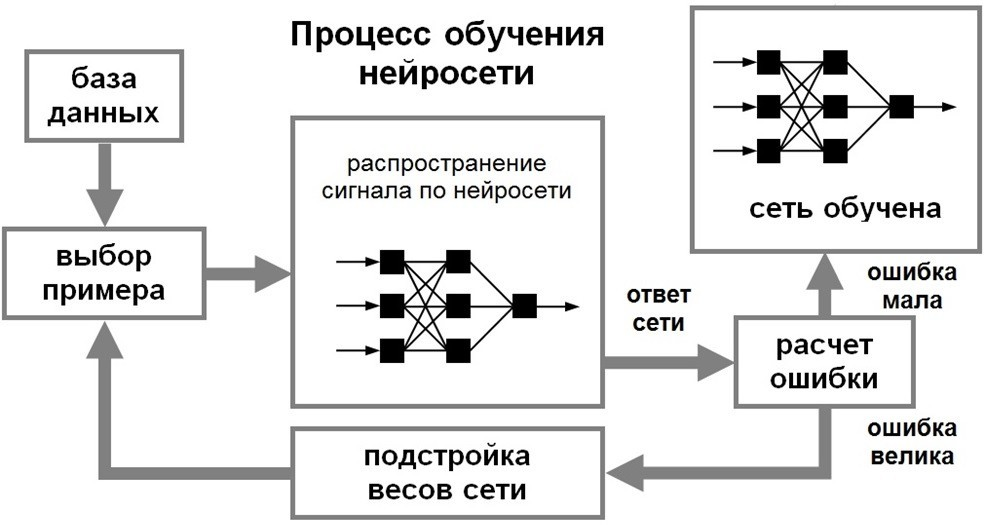
\includegraphics[width=0.8\textwidth]{images/sxema.jpeg}
	\caption{Архитектура нейронной сети с одним скрытым слоем}
	\label{fig:neural_network}
\end{figure}
	
	\section{Математическая постановка задачи}
	
	\subsection{Стандартный градиентный спуск}
	
	Классический метод градиентного спуска для минимизации функции \texttt{$J(\theta)$} определяется следующей итерационной формулой:
	
	\begin{equation}
		\label{eq:gd}
		\theta_{t+1} = \theta_t - \alpha \nabla J(\theta_t)
	\end{equation}
	
	где $\nabla J(\theta_t)$ — градиент функции потерь в точке $\theta_t$.
	
	\subsection{Стохастический градиентный спуск}
	
	В отличие от пакетного метода, SGD использует один случайный пример для оценки градиента:
	
	\begin{equation}
		\label{eq:sgd}
		\theta_{t+1} = \theta_t - \alpha \nabla J_i(\theta_t)
	\end{equation}
	
	где $i$ — индекс случайно выбранного обучающего примера [2].
	
	\subsection{Метод Адама (Adam)}
	
	Алгоритм Adam сочетает преимущества RMSprop и Momentum:
	
	\begin{equation}
		\label{eq:adam}
		\theta_{t+1} = \theta_t - \frac{\alpha}{\sqrt{\hat{v}_t} + \epsilon} \hat{m}_t
	\end{equation}
	
	где $m_t$ и $v_t$ — оценки первого и второго моментов градиента [3].
	
	\section{Экспериментальные результаты}
	
	В таблице~\ref{tab:comparison} представлено сравнение скорости сходимости различных методов оптимизации.
	
	\begin{table}[H]
		\centering
		\caption{Сравнение методов градиентного спуска}
		\label{tab:comparison}
		\begin{tabular}{|c|c|c|c|}
			\hline
			\textbf{Метод} & \textbf{Итераций до сходимости} & \textbf{Время (сек)} & \textbf{Точность} \\
			\hline
			GD & 1000 & 45.2 & 0.892 \\
			\hline
			SGD & 800 & 12.5 & 0.875 \\
			\hline
			Adam & 300 & 8.3 & 0.901 \\
			\hline
		\end{tabular}
	\end{table}
	
	На рисунке~\ref{fig:learning_curve} показаны кривые обучения для трёх методов.
	
	\begin{figure}[H]
		\centering
		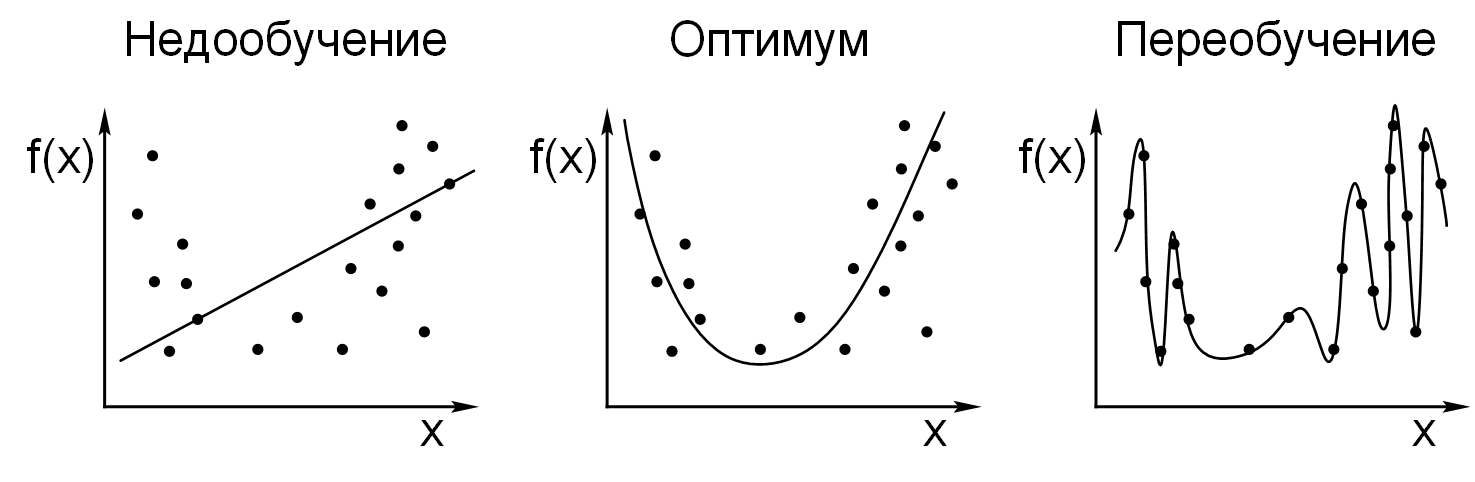
\includegraphics[width=0.8\textwidth]{images/grafik.png}
		\caption{Кривые сходимости методов оптимизации}
		\label{fig:learning_curve}
	\end{figure}
	
	\section{Реализация алгоритмов}
	
	Ниже представлена реализация метода градиентного спуска на языке \texttt{Python} с использованием библиотеки \texttt{NumPy}.
	
	\subsection{Код на Python}
	
	\inputminted{python}{code/example1.py}
	
	\subsection{Код на C++}
	
	\inputminted{cpp}{code/example2.cpp}
	
	\subsection{Пояснение к коду}
	
	В листинге~1 функция \texttt{gradient\_descent} принимает параметры:
	\begin{itemize}
		\item \texttt{X} — матрица признаков;
		\item \texttt{y} — вектор целевых значений;
		\item \texttt{alpha} — скорость обучения;
		\item \texttt{num\_iters} — количество итераций.
	\end{itemize}
	Вычисления градиента выполняются с использованием векторизации, что повышает производительность.
	
	\section{Заключение}
	
	В ходе работы были рассмотрены три модификации метода градиентного спуска. 
	Экспериментально подтверждено, что метод Adam [3] достигает наилучшей скорости сходимости (300 итераций) и точности (0.901) по сравнению с классическим GD и SGD.
	
	\section*{Список источников}
	\addcontentsline{toc}{section}{Список источников}
	
	\begin{enumerate}[label={[\arabic*]}]
		\item Goodfellow I., Bengio Y., Courville A. Deep Learning. — MIT Press, 2016.
		\item Bottou L. Large-Scale Machine Learning with Stochastic Gradient Descent // Proceedings of COMPSTAT'2010. — Springer, 2010. — P. 177–186.
		\item Kingma D.P., Ba J. Adam: A Method for Stochastic Optimization // arXiv preprint arXiv:1412.6980, 2014.
	\end{enumerate}
	
\end{document}